\section{Methodology}


\label{method}

\subsection{Overview}
We implement both SimCLR and RotNet frameworks using a ResNet-20 backbone encoder applied on the CIFAR-10 dataset to increase comparability between the two frameworks. Our ResNet-20 encoder has three residual blocks of three convolutional layers each. We also use the vanilla ResNet-20 model as a supervised baseline model to benchmark performance. However, due to the different nature of the frameworks, we proceed to lightly tune hyper-parameters of our model, including \texttt{batch\_size}, \texttt{lr\_decay}, \texttt{optimizer}, \texttt{num\_epochs}, separately in order to achieve the best performance we can given our computational limitations. 

\subsection{SimCLR}

\subsubsection{The Contrastive Learning framework}
Contrastive learning has been shown to be a powerful approach for learning visual representations from large amounts of unlabeled data. The core idea behind contrastive learning is to use pairs of similar and dissimilar images to learn a representation that captures the differences between the images in the pair.

This framework has the following major components:

\begin{enumerate}
    \item A stochastic data augmentation module that transforms any input image into a pair of correlated views, $\mathbf{x_i}$ and $\mathbf{x_j}$ of the same input, which we call a positive pair. We sequentially apply a random resized crop, followed by a random color distortion. 
    \item The ResNet-20 base encoder network $F(\cdot)$, which extracts features from the input images and encodes them into a lower-dimensional latent space.
    \item A 2-layer MLP projection head $G(\cdot)$, which maps the latent representations to a higher-dimensional space.
    \item A contrastive loss function, which is defined for a positive pair in the following manner:
    $$ l_{i,j} = - log \frac{exp(sim(\mathbf{z_i},\mathbf{z_j})/\tau}{\sum_{k=1}^{2N} \mathbbm{1}_{[k \neq i]} exp(sim(\mathbf{z_i},\mathbf{z_j})/\tau)}$$
    where $sim(\mathbf{u},\mathbf{v}) = \mathbf{u}^\top \mathbf{v}/||u|| ||v||$ and $\tau$ denotes a temperature parameter. The indicator function $\mathbbm{1}_{[k \neq i]}$ evaluates to 1 iff $k \neq i$.
\end{enumerate}

% Insert image of SimCLR architectural diagram
\begin{figure}[!htbp]
    \centering
    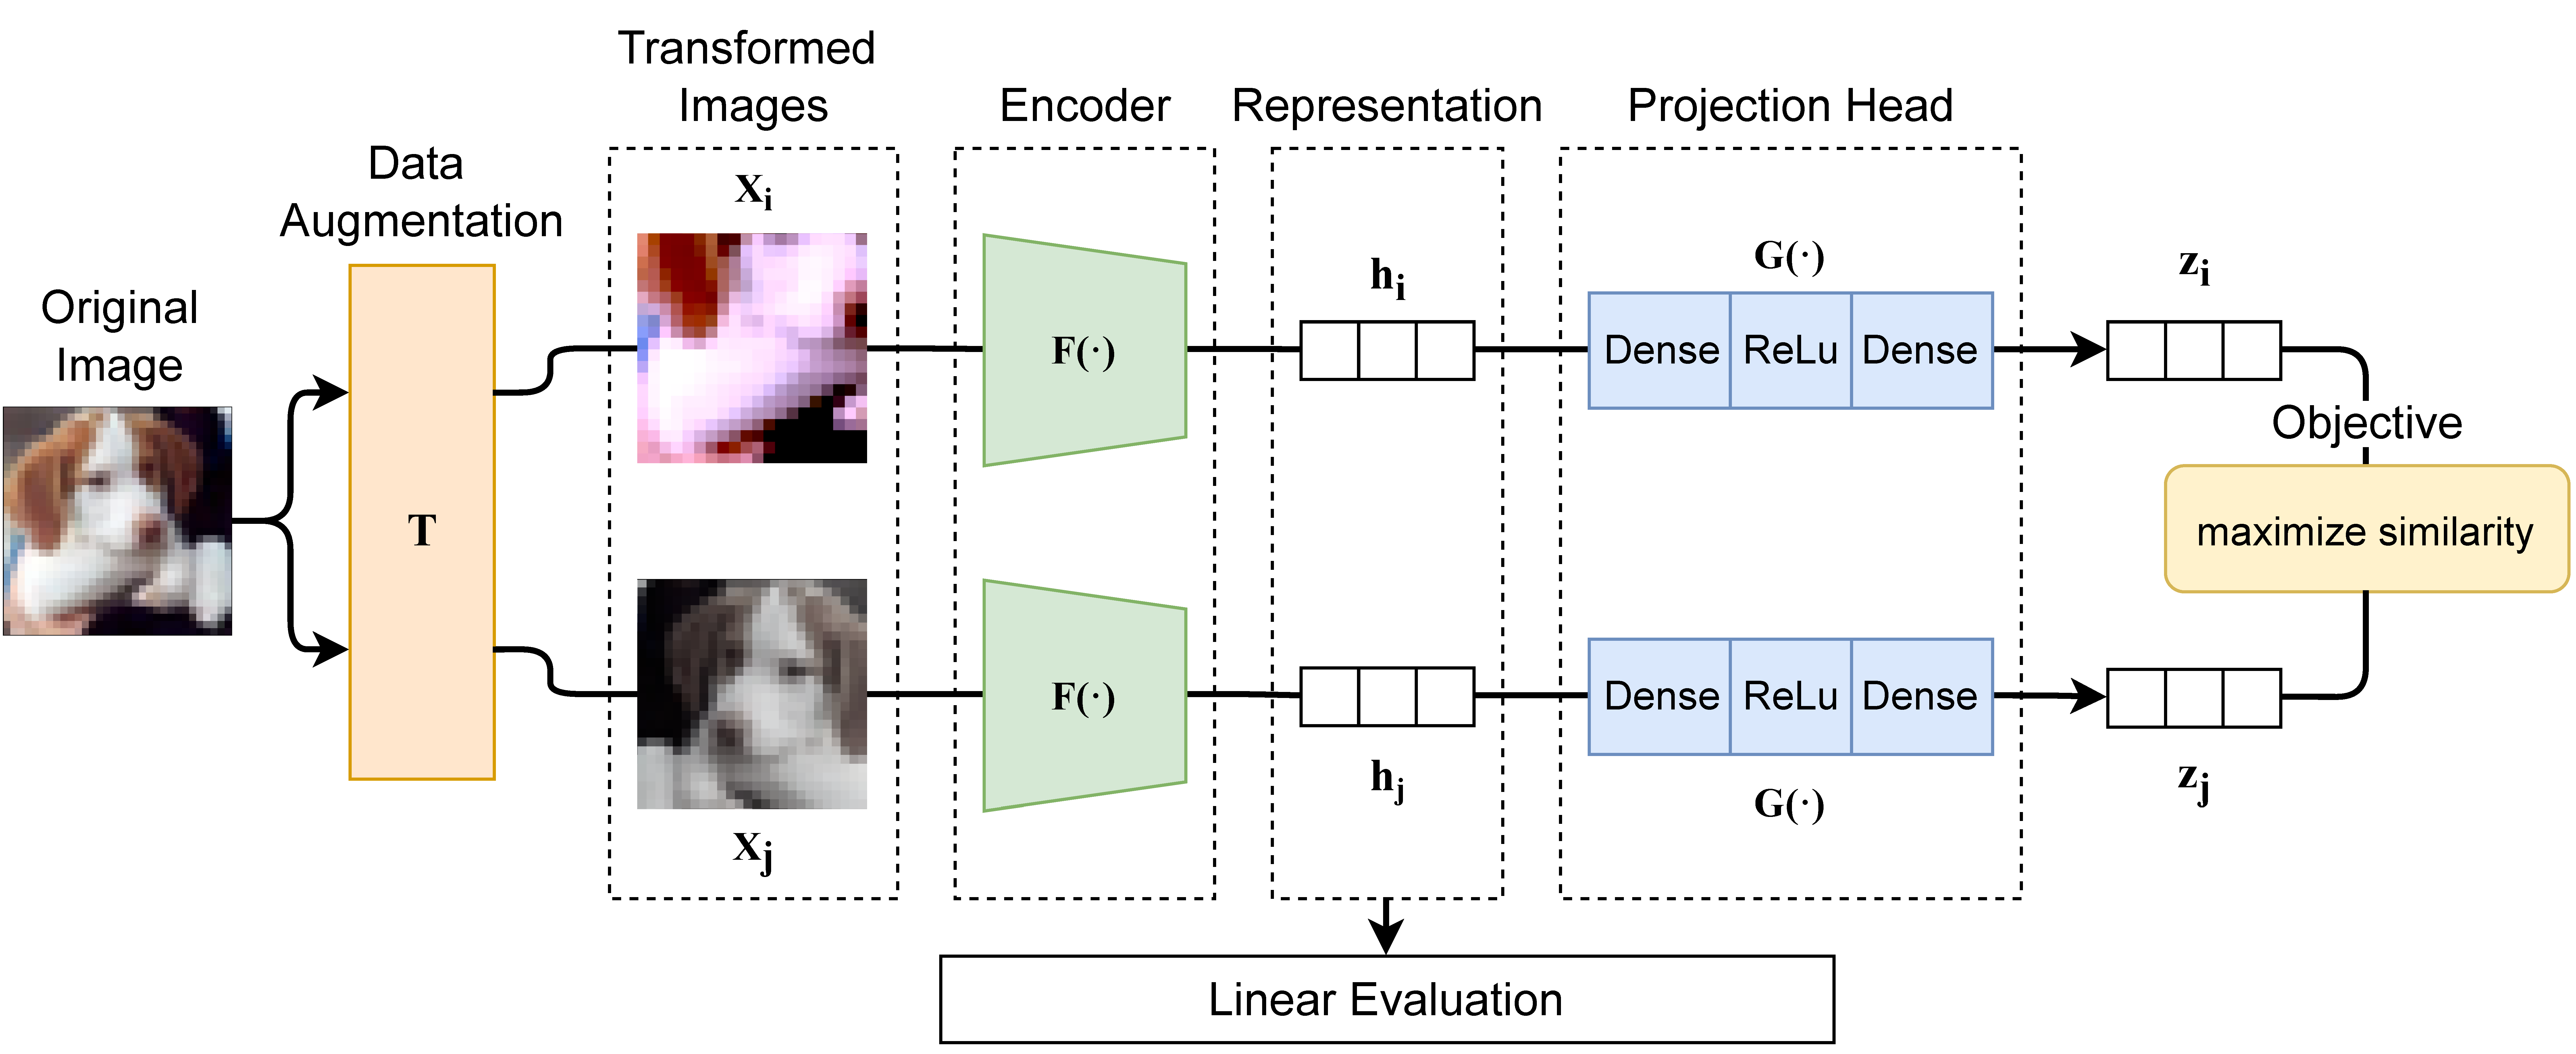
\includegraphics[width=1\linewidth]{figs/archDiag_SimCLR.png}
    \caption{Architectural diagram of SimCLR framework}
    \label{fig:archDiag_SimCLR}
\end{figure}

\paragraph{Hyper-parameters} For our implementation, we used the following settings: \texttt{EPOCHS=100}, \texttt{BATCH\_SIZE=1024}.

We optimized a temperature-scaled cross entropy-loss using a LARS optimizer with a learning rate of 0.012 and a weight decay of $1\mathrm{e}{-6}$. Further, we use a linear warm-up for the first 20 epochs, and decay the learning rate with the cosine decay schedule.

\subsection{RotNet}

The RotNet framework from paper \cite{RotNet} involves two primary steps to perform classification tasks: 1) unsupervised training on rotated images to predict its rotation and 2) semi-supervised fine-tuning process on the pre-trained unsupervised model using labeled data to classify images.

\subsubsection{Unsupervised model}

We rotate each input image (by $0^0$,$90^0$,$180^0$,$270^0$), assign labels according to its rotated angel, and train a ConvNet to learn representations of transformed input images. To effectively predict image rotations, the ConvNet must first learn to identify and locate important objects (i.e. dog's ears) in images to understand their context. It must also understand how different types of objects are typically depicted in the input images and use this information to relate the position of the objects to the dominant orientation of the image.

% Insert image of RotNet architectural diagram
\begin{figure}[!htbp]
    \centering
    
\includegraphics[width=.80\linewidth]{figs/archDiag_RotNet.png}
    \caption{Architectural diagram of RotNet framework}
    \label{fig:archDiag_RotNet}
\end{figure}

\paragraph{Hyper-parameters} For our implemention, we used the following settings: \texttt{EPOCHS=100}, \texttt{BATCH=128}, \texttt{INITIAL\_LR=0.1}, \texttt{DECAY=0.2}, \texttt{DECAY\_EPOCHS=[30, 60, 80]}. 

\subsubsection{Semi-supervised}

The architecture of the semi-supervised model is the same as the unsupervised model, except that the fully connected layer has an output size of 10 for image classification from CIFAR10.

\subsection{Evaluation Process}

To evaluate our model performance we applied linear evaluation protocol on both SimCLR and RotNet encoders. Linear evaluation one of the intended methods to evaluate model performance in the SimCLR paper \cite{SimCLR}, where we load the representations learned by the encoder, freeze all weights, and train one added linear layer with labeled data (texttt{out\_features = 10}) to classify images. It is difficult to find a fair comparison for SimCLR linear evaluation in RotNet due to the different intended use of the RotNet model for downstream tasks. Therefore, we evaluate the RotNet encoder both with the same linear process as SimCLR as well as with the intended semi-supervised setting from the RotNet paper \cite{RotNet}. Semi-supervised setting involves loading the trained encoder model, freezing only the first residual block(s), and retraining the latter block(s) with a fully-connected layer (texttt{out\_features = 10}) on labeled data.

One goal of this project is to understand how the SimCLR and RotNet frameworks perform on image classification tasks when we have partially labeled data. Therefore, we train our evaluation models on only 1\% and 10\% of our labeled data (50 images and 500 images per class respectively).

For linear evaluations, we trained the fully-connected layer over 90 epochs as instructed in the paper \cite{SimCLR} on 1\% and 10\% labels. For the RotNet semi-supervised setting, we froze the first two residual blocks of encoder and retrained the last over 80-100 epochs.



% #######
% Our goal is to train an unsupervised network using the RotNet method, and then first evaluate its performance on a classification problem with fine tuning of a fully connected layer and comparing these results with the performance of SimCLR, and then perform self-supervised training using this network with fine-tuning of the residual blocks.
% #######


